\chapter{红外图像无人机目标检测相关理论}

\section{人工神经网络}
人工神经网络又称为类神经网络,一般简称神经网络。在机器学习领域中是一种模仿生物的神经网络结构的计算模型。这种模型常常被用来估计一种未知的函数。神经网络由大量的传输节点构成,这些传导节点也可以称为人工神经元。这些节点往往由若干个参数进行定义,这些参数就称为模型的权重。这些权重能够借助外界的信息对自身的值进行更新,也就是模型具备学习功能。在很多领域,神经网络能有类似人类的决定能力,因此很多传统编程方法难以解决的问题都可以用神经网络来进行解决。

一般意义上的神经网络主要由三个部分组成:结构、激活函数和学习规则。
结构主要指的是网络中的各种节点的计算方法和各节点之间的关系,一般指的是网络的权重。激活函数指的是将神经网络中某一层的计算结果进行某种的特定运算来扩大网络拟合结果的范围,提升网络对目标函数的拟合能力。学习规则指的是网络通过训练更新参数的具体策略。

\section{卷积神经网络}
卷积神经网络的主要特点是引入了卷积操作,通俗地说,卷积操作就是对输入的某个向量应用某种向量乘法,这种卷积操作对于提取某个区域的整体信息有较好的效果,因此在目标检测、图像分类、自然语言处理等计算机视觉任务中基于卷积神经网络的算法都能取得更好的性能。一般情况下卷积神经网络的主要组成如图\ref{cnn}所示,
卷积神经网络按照推理计算的顺序可以分为输入端、卷积层、池化层、全连接层等部分。

\begin{figure}[htbp]
    \centering
    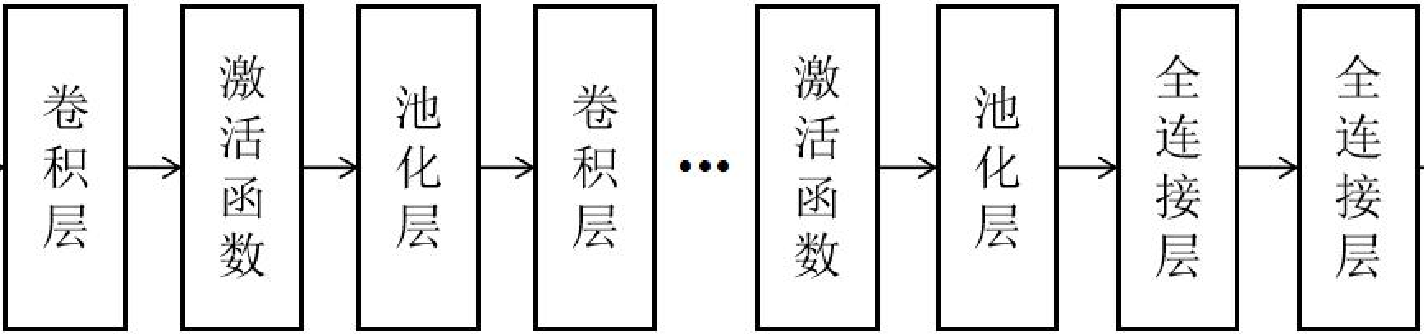
\includegraphics[width = 0.9\textwidth]{cnn.png}
    \caption{卷积神经网络常见结构}
    \label{cnn}
\end{figure}

下文将对卷积神经网络的各个主要组成部分进行介绍。

\subsection{卷积层}
卷积层的作用是定义一种卷积的运算方法。该层的权重参数经过训练后就用来对输入图像等张量进行特定的卷积运算,一般的作用是提取出重要特征。
通常卷积运算的公式可以写成如式\ref{conv1}所示:
\begin{equation}
    \mathrm{s}(t)=\left(x^{*} w\right)(t)
    \label{conv1}
\end{equation}

\begin{figure}[htbp]
    \centering
    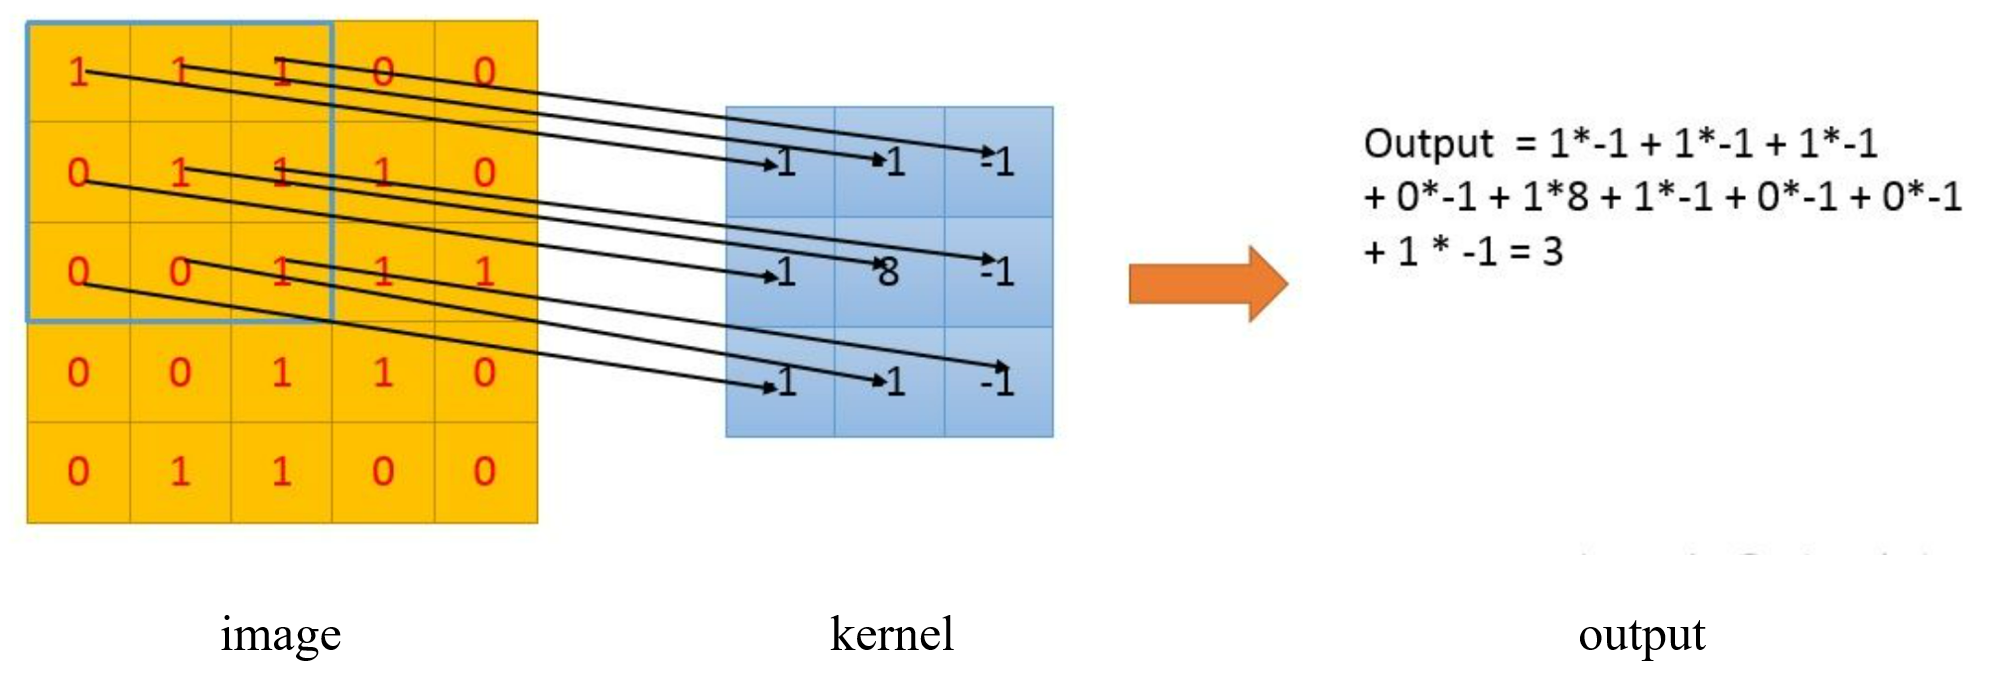
\includegraphics[width = 0.9\textwidth]{jjgc.png}
    \caption{图像卷积运算过程}
    \label{jjgc}
\end{figure}

式中$x$代表输入张量,$w$ 代表定义卷积核的函数。
对于在图像中的卷积运算,卷积核和输入图像之间的卷积运算可以视为矩阵乘法,因为卷积核的大小往往比输入图像小很多,卷积操作往往是一种提取图像局部特征的操作。
对图像的卷积过程如图\ref{jjgc}所示,
假设输入图像经过处理后可以视为$5\times5$的矩阵,卷积核的尺寸为
$3\times3$,卷积操作的具体过程就是从图像的左上角往右下角遍历,在每一次的遍历过程中将输入图像和卷积核进行比对,将输入图像和卷积核上对应位置的值进行相乘之后累加起来,每一次卷积核的运算对应一个运算结果,该运算结果是一个标量,并且根据卷积核的运算轨迹,该运算结果也将填在总体的卷积运算结果对应的输出矩阵的对应位置上。
卷积运算输出特征图的尺寸由式\ref{cout}决定,
\begin{equation}
    N_{\text {output }}=\frac{\left(W_{\text {input }}-F+2 P\right)}{S}+1
    \label{cout}
\end{equation}

式中,$W$代表输入图像的尺寸,$F$ 表示卷积核的尺寸, $P$ 表示 padding 填充的像素个数,$S$ 代表卷积核移动的步长。
通过训练,可以更新卷积核的参数,最理想的训练达到的效果是每个卷积核都完美地拟合到它们各自应该具备的功能上,比如提取目标的边缘、提取目标的某种形态等。这样整个卷积神经网络中的卷积核相互协作,共同完成整个系统应该具备的算法功能,并且取得较好的性能。卷积神经网络的核心思想就是通过训练使得网络中的各个卷积核具备最接近最佳算法的参数权重,从而达到拟合出处理输入对象的正确目标函数的目的。

\subsection{激活函数}
激活函数的主要作用是解决非线性问题。在神经网络的推理计算过程中,由于计算基本上由线性加权运算组成,因此运算的结果往往缺乏对非线性目标函数的拟合性能,这时就需要引入激活函数来增强网络的非线性。
常用的激活函数如下:

(1)Sigmoid 函数:Sigmoid函数也称Logistic 函数,是一种典型的激活函数,该函数的数学定义式可以写作如式\ref{log}所示,
\begin{equation}
    \sigma(x)=\frac{1}{\exp (-x)+1}
    \label{log}
\end{equation}

\begin{figure}[htbp]
    \centering
    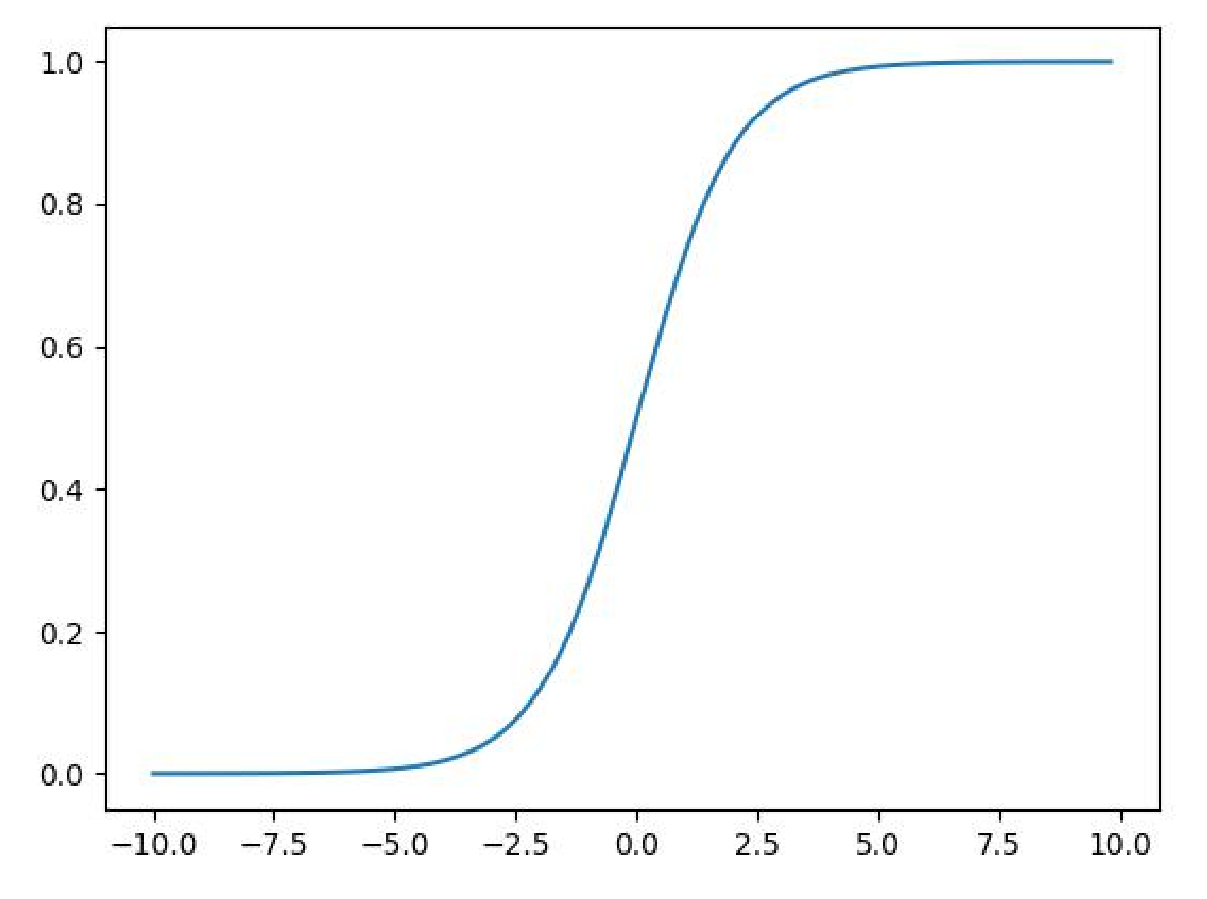
\includegraphics[width = 0.5\textwidth]{sigmoid.png}
    \caption{Sigmoid函数}
    \label{sig}
\end{figure}

\begin{figure}[htbp]
    \centering
    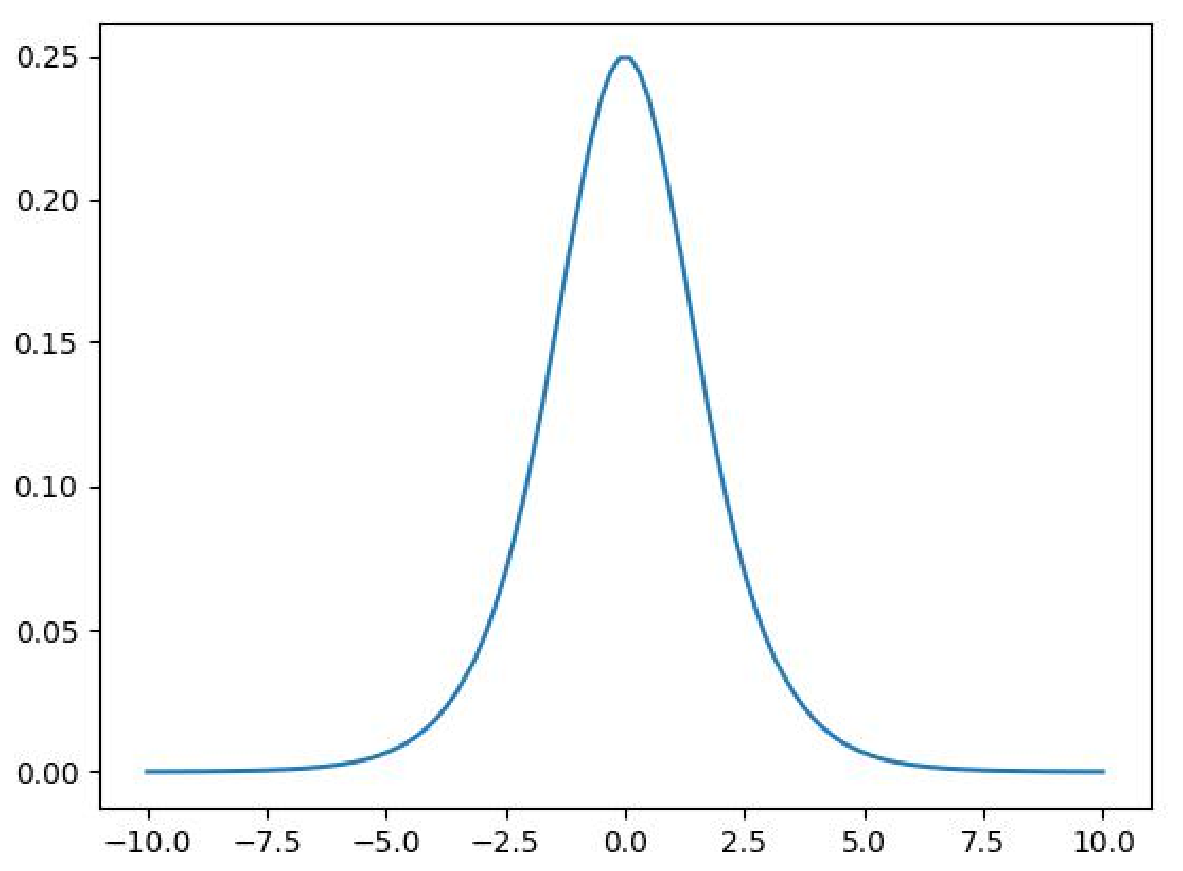
\includegraphics[width = 0.5\textwidth]{sig导数.png}
    \caption{Sigmoid导函数}
    \label{sigd}
\end{figure}

Sigmoid函数的图像如图\ref{sig}所示,由该图像可知,在输入Sigmoid函数系统处理后,输出的范围在$[0,1]$,因此该函数可以应用于二分类任务。Sigmoid函数的导数如图\ref{sigd}所示,从图中可知,
Sigmoid函数的微分容易计算,但是Sigmoid函数存在的问题是但输入不在特定范围内时会出现“梯度消失”的情况,影响模型的训练效果。针对这种梯度消失的问题,后续的研究人员提出了ReLU函数。

(2)Tanh 函数:Tanh 函数又叫做双曲正切激活函数,该函数的主要贡献是一定程度上解决了Sigmoid函数中存在的均值问题。Tanh函数的定义式如式\ref{tanh}所示,Tanh函数的图像如图\ref{tanh}所示,
由图\ref{tanh}可知,输入数据在经过Tanh函数的处理后输出范围是$[-1,1]$,并且该函数的图像在直角坐标系中是以原点为中心呈中心对称的,因此可以将Tanh函数视为Sigmoid函数经过平移和拉长的改进版本。虽然Tanh函数在实验中的性能相比Sigmoid函数有所提升,但是梯度消失的问题仍然存在。

\begin{equation}
    \sigma(x)=\tanh (x)=\frac{\exp (x)-\exp (-x)}{\exp (x)+\exp (-x)}=2 \operatorname{sigmoid}(2 x)-1
    \label{tan}
\end{equation}

\begin{figure}[htbp]
    \centering
    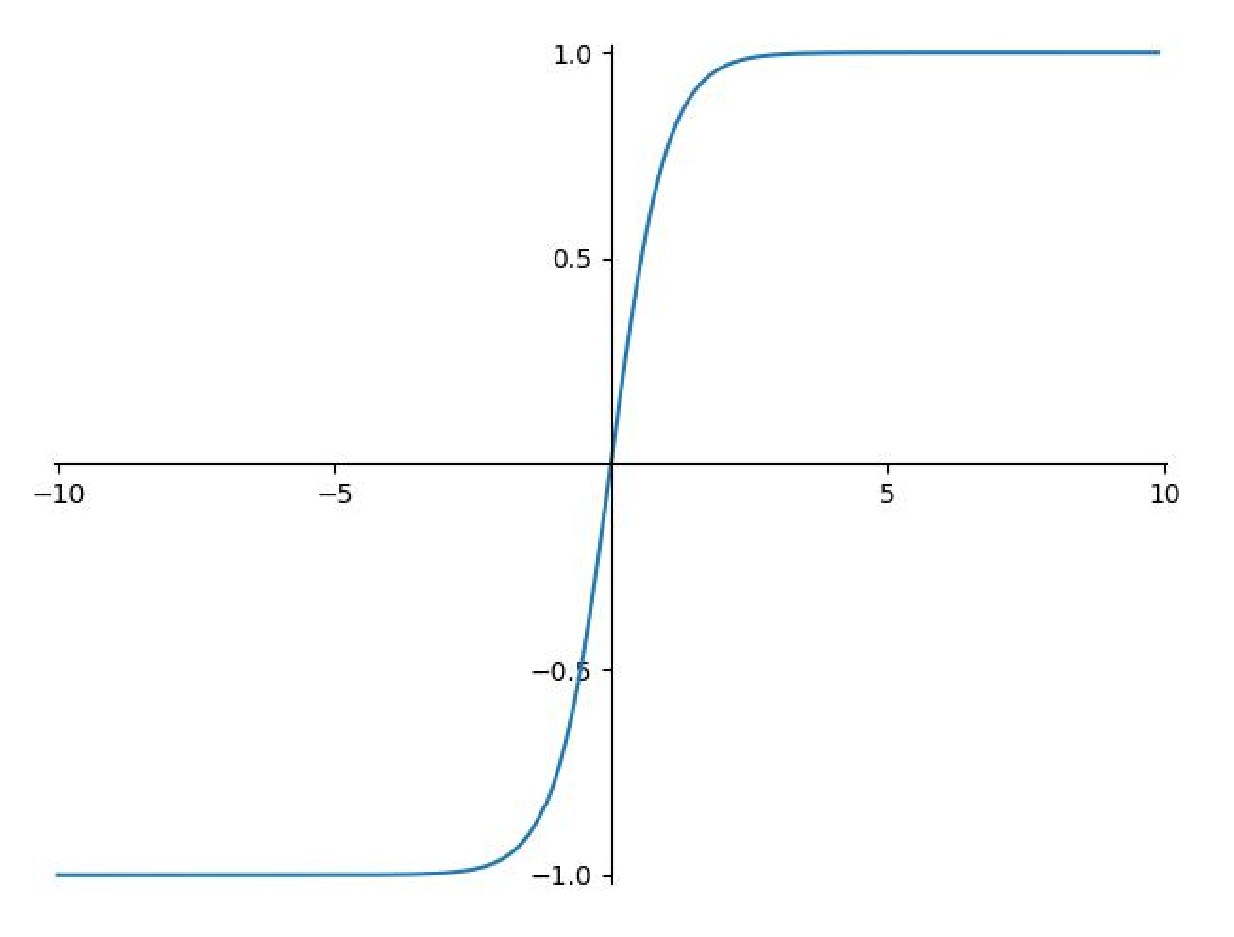
\includegraphics[width = 0.5\textwidth]{tanh.png}
    \caption{Tanh函数}
    \label{tanh}
\end{figure}

(3)ReLU 函数:ReLU函数的定义可以写作如式\ref{relu}所示,2010 年
Hinton 和 Nair 等人经过对神经网络结构的研究和分析,提出了ReLU函数。从ReLU函数的导函数中可知, ReLU 函数具备在$x\ge 0$时导数值为 $1$的特性,因此ReLU函数有对梯度消
失现象进行了有效的处理,这也使得ReLU函数成为了各类卷积神经网络中最常用的激活函数之一\cite{xu2015empirical}。ReLU函数和上文提到的Sigmoid函数和Tanh函数的主要区别是,该函数的定义式十分简单,在实际运算过程中也具备很快的计算速度。但ReLU函数的主要问题是将$ x<0$的部分
强制输出$0$,这中处理方法可能会导致“死区”问题,因此后续的研究人员提出了LeakyReLU\cite{maas2013rectifier}等改进版本。

\begin{equation}
    \sigma(x)=\max (0, x)= \begin{cases}x & x \geq 0 \\ 0 & x<0\end{cases}
    \label{relu}
\end{equation}

\subsection{池化层}
卷积网络的一个典型的模块组合方式是卷积、激活和池化。具体的流程是首先通过卷积层上的各个卷积核对输入特征图进行卷积运算,得到输出的特征图,在得到卷积产生的特征图后将结果输入激活函数中,将输出的特征进行激活处理,激发网络计算的非线性,最后一步就是池化操作,主要作用是将卷积和前序模块提取的特征进行合并和稀疏化,从而增强网络对整体特征的感知能力,同时减少网络的运算量。
最大池化运算的主要过程如图\ref{maxp}所示。
实际的卷积神经网络应用中,经常使用的池化方法主要有最大池化、平均池化等。
一般情况下,卷积神经网络池化层的主要功能可以归纳为以下几点:

(1)目标特征形态不变性。
由于池化过程一般是以某个区域内的某个点作为池化层的输出,所以即使该点在该区域中
产生了一定程度的位移,只要位移后的位置仍然位于该区域内,池化层输出的特征向量就不会受到影响,因此从具体意义上来看,图像上的某个特征点就算产生了一些位移,对于池化层来说这种位移是不对输出产生影响的。

(2)降低输出特征图的维度。
池化运算相当于对输入特征图以一定规则进行了缩小,得到的输出图像就是输入特征图的某些像素点重新拼接后组成的特征图,因此也称为降采样过程。

(3)池化层的处理导致的必然结果是降低整个模型的计算量和参数量,包括池化层后续的模块的参数量,因此也对解决过拟合问题有所贡献\cite{gu2018recent}。

\begin{figure}[htbp]
    \centering
    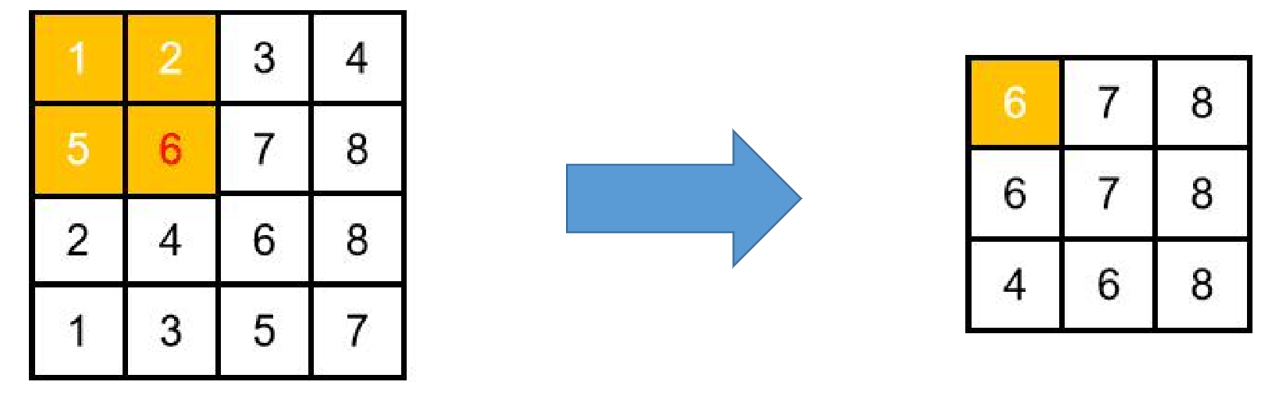
\includegraphics[width = 0.9\textwidth]{maxp.png}
    \caption{最大池化示意图}
    \label{maxp}
\end{figure}

\subsection{全连接层}
全连接层在经典的全连接网络中比较常见,在卷积神经网络中,通常采用少量的全连接层,对前序的卷积层等模块所提取出的图像目标特征等信息进行整合和判决,从而输出整个算法的最终结果。但是全连接层一般接收的输入张量大小是固定不变的,所以实际算法应用中往往采用卷积层来替代全连接层,组成全卷积网络,用卷积层进行网络的输出同样可以起到整合结果、得出结论的作用。

\section{目标检测的评价指标}
在绝大多数研究中,目标检测算法的性能通常可以由两个指标来进行衡量和比较,即
平均准确度均值(the mean
Average Precision,mAP)
和FPS(Frames per second)。

mAP主要由两个方面组成,分别是模型的精确率(Precision)和召回率(Recall)。通俗地说,优秀的目标检测精度就是指精确率和召回率都能处在较高水平。平均准确度就是指综合考虑精确率和召回率之后得出的性能表现,而均值指的是目标检测中每个待测目标类型都会得出一个平均准确度,平均准确度均值就是将这若干个平均准确度进行算术平均后得到的值。AP(Average-Precision)的具体计算方法是根据算法对整个测试集的所有图像进行的预测计算召回率和精确率,并将每一个召回率对应的最大精确率的值同时在一个直角坐标系内描点,在连线后求该曲线和坐标系包围的区域的面积。直观地,精确率和召回率都较高的模型能获得更高的AP值。
下面介绍与 AP 相关指标的概念。

(1)IoU:衡量模型计算得出的预测框和真值框之间的匹配程度的一种标准,主要计算方法是将预测框和真值框的相交部分面积和这两个部分的相并区域面积作比,如果IoU值较高,就认为模型对目标的定位能力较强,对于检测任务来说,一次成功的检测往往要求预测框和真值框的IoU大于某个标准,如$0.5$等。

(2)True和False、Positive和Negative:True或是False指的是模型得出的判断对照真值后可知是正确的判断或是错误的判断,而Positive或是Negative指的是模型算法对某个区域的计算结果是认为该区域有某种类型的目标,或是模型不认为该区域有某种类型的目标。具体地,True Positive指的是模型对该区域做出的判断是有某种类型的目标,而经过和真值框的对照,该区域确实存在该类型的目标,模型的判断结果正确。True Negative是指模型的判断是该区域不存在某类型目标,真值中确实也不存在该类型目标,模型的判断结果正确。False Positive指的是模型的判断结果是该区域存在某类型目标,但是真值中该区域不存在该类型目标,模型判断错误。False Negative是指模型判断该区域存在某类型目标,但是真值中存在该类型目标,因此模型判断错误。
在计算量化时,通常将TP、TN、FP、FN表示成符合上述情况的示例的数量。

(3)精确率:精确率的定义式如
式\ref{pr}所示。精确率表示模型判断出存在的目标数量且验证未正确的数量占模型判断出的所有目标的比例,衡量的是模型做出的判断中有多少是准确的。

\begin{equation}
     \text { Precision }=\frac{T P}{T P+F P}
    \label{pr}
\end{equation}

(4)召回率:召回率的定义式如
式\ref{rec}所示。召回率表示模型判断出的目标数量和真值中总共存在的所有目标数量的比值,表示真值中的样本有多少被模型计算找出,衡量模型对目标的发现能力。

\begin{equation}
     \text { Recall }=\frac{T P}{T P+F N}
    \label{rec}
\end{equation}

在设置了固定的IoU门限后,很容易测出对应的精确率和召回率曲线。常用的数据集可能会因为对IoU门限的设置而存在各自不同的计算规则。具体地,VOC 2007数据集选择的IoU门限是0.5,而 MS COCO的处理方式是计算IoU门限值在[0.5,0.95]之间以$0.5$为步长每$0.5$选定一个IoU进行测试,从而测出10组数据,求这10组数据的平均值。本文采用的方式和VOC 2007相同,也称为mAP@0.5。

FPS这一指标一般用于衡量目标检测算法的速度,通过衡量算法每秒可以处理的图像数量也就是求每张图像处理耗时的倒数。这一指标往往应用于对实时检测要求更高的任务中,在实际的工程应用中对算法和移动设备的实时检测能力要求较高,因此以YOLO系列为代表的单阶段目标检测算法因为能在FPS这一指标上取得较好的表现而得到广泛的应用。

\section{红外成像原理}
传统上,红外技术与控制功能和夜视问题有关,早期的应用仅与探测红外辐射相联系,后来通过形成红外图像
,形成温度和发射率差异\cite{rogalski2002infrared}。现代红外技术的起源于第二次世界大战期间。最近在将红外技术应用于遥感问题方面取得的成功是由于近50多年来对高性能红外探测器的成功开发。大部分资金已用于满足军事需要,但民用应用不断增加,特别是在20世纪的最后10年。这些应用包括医疗、工业、地球资源和节能应用。医学应用包括热成像,其中人体的红外扫描可以用于检测癌症或其他提高体表温度的创伤
。此外,地球上各种资源的确定可以通过使用来自卫星的红外图像与现场观察的校准。在某些情况下,甚至一种作物的健康状况也可以从太空中借助红外探测得到确定。利用红外扫描来确定最大热损失点,帮助了家庭和工业的节能。由于这些技术的有效应用,在全球环境污染和气候变化监测、农业作物产量的长期预测、化学过程监测、傅里叶变换红外光谱学、红外天文学、汽车驾驶、医学诊断中的红外成像等方面,使用这些技术的需求正在迅速增长。

红外目标检测可以分为图像预处理和目标检测两个步骤,因此在进行后续工
作前需要分析红外图像的获取过程以及红外图像存在的特性。本节从红外成像的理论基础、红外成像的过程、红外图像的特性等方面进行相关概念的介绍,为后续工作开展打下理
论基础。
\subsection{物体的热辐射}
红外成像和探测的基础是物体的热辐射。
根据物体固有的物理特性,微观上很多尺寸特别微小的原子组合在一起成为了一个个物体,而这些物体在不断地进行振动,当某些原子自身的能量较大时,往往振动所表现出的能量也更大。宏观上整个物体的原子振动和其自身的温度有关,温度高的物体原子振动较快,辐射出的光谱能量也更大。综上所述,每个物体都在不断向外界发射热辐射,这种辐射往往以红外线的形式存在,这种辐射的量化采用引入黑体的方式。
黑体的辐射功率(或发射的光子数)及其波长分布可以由普朗克辐射定律给出,如式\ref{plank1}和式\ref{plank2}所示。
\begin{equation}
    W(\lambda, T)=\frac{2 \pi h c^{2}}{\lambda^{5}}\left[\exp \left(\frac{h c}{\lambda k T}\right)-1\right]^{-1} \quad \mathrm{~W} /\left(\mathrm{cm}^{2} \mu \mathrm{m}\right)
    \label{plank1}
\end{equation}

\begin{equation}
    P(\lambda, T)=\frac{2 \pi c}{\lambda^{4}}\left[\exp \left(\frac{h c}{\lambda k T}\right)-1\right]^{-1} \text { photons } /\left(\mathrm{s} \mathrm{cm}^{2} \mu \mathrm{m}\right)
    \label{plank2}    
\end{equation}

其中$\lambda$表示波长,$T$表示温度,$h$是普朗克常数,$c$是光速,$k$是玻尔兹曼常数。

\subsection{红外成像过程}

红外线和生活中常见的可见光、紫外线一样,属于一种电磁波。红外线的波长处在$760nm$到$1mm$之间,红外线的波长比可见光更大,比微波更小。根据上文所述,理论上所有物体都会向周围的环境发射红外辐射。而对应地,红外成像系统就是一种采集周围物体所发射的红外辐射的设备,并将这种辐射量化成像后以图像的形式进行表达。
红外成像技术原理如图\ref{infra}所示\cite{倪国强2008中国红外成像技术发展的若干思考}。

\begin{figure}[htbp]
    \centering
    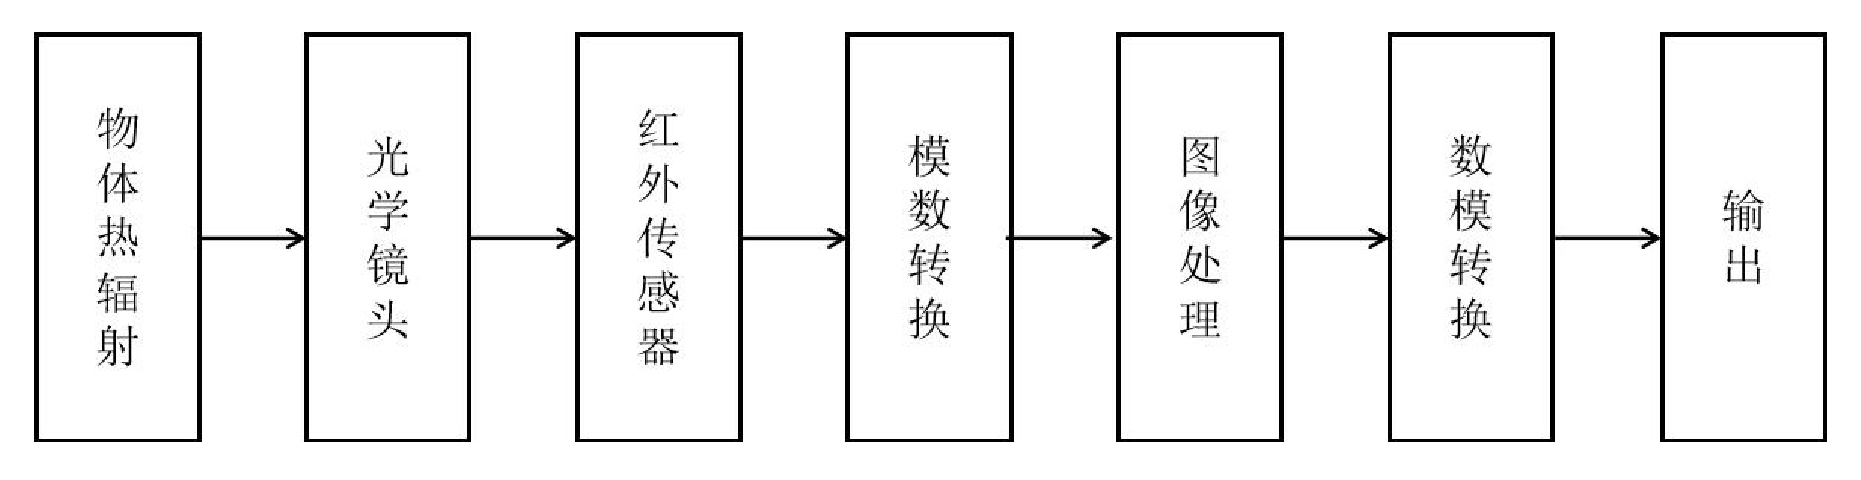
\includegraphics[width = 0.9\textwidth]{红外成像.png}
    \caption{红外成像过程示意图}
    \label{infra}
\end{figure}

如图\ref{infra}所示,常规的红外成像系统的成像流程是,从红外摄像机对目标区域的红外辐射进行感知,这一部分需要将外界的红外辐射进行采集后进行模拟-数字转换,转换后格式化为图像形式,之后就可以应用各种算法对采集到的红外图像进行处理。

\subsection{红外图像特性} 

本文研究了红外成像系统的应用场景、红外成像系统的硬件条件、红外成像的自然环境等因素,分析得出红外图像的主要特点有:

(1)红外图像的质量较低。由于红外成像系统成像需要依靠接收外界发射的红外辐射,这种辐射能量在空气环境中传输会遇到各种损耗,从而影响最终的成像质量,具体表现为分辨率、对比度较低。

(2)红外图像一般信噪比较低。
红外成像系统在接收外界的红外辐射时,向所有目标区域内物体进行探测,不可避免地会遇到周围设备的噪声,红外成像设备的固有特性导致其产生光子噪声等噪声,此外还有各种环境噪声,使得红外成像系统采集到的红外辐射图像往往信噪比不高。

(3)红外图像中物体边缘不清晰。相互之间距离较近的物体可能会对彼此的红外辐射产生影响,所以这时对这些物体的红外辐射进行探测后得到的红外图像中往往物体间的边缘不够明显,这样的特性也会不利于后续的目标检测等处理。

\section{本章小结}
本章主要是对研究本课题需要的基础理论知识进行了介绍。本章首先介绍了人工神经网络的定义,之后对组成卷积神经网络的常见模块如卷积层、池化层的定义和计算方法做了详细的介绍,而后对本课题研究的目标检测算法的性能评价指标进行了介绍。最后,介绍了本课题研究的红外图像的成像过程的相关基础知识,后续对红外图像特性的分析和利用就是从红外图像成像的各种特点入手,从而抓住问题的关键,针对性地设计处理红外图像的算法,最终提升红外图像无人机目标检测算法的性能。


